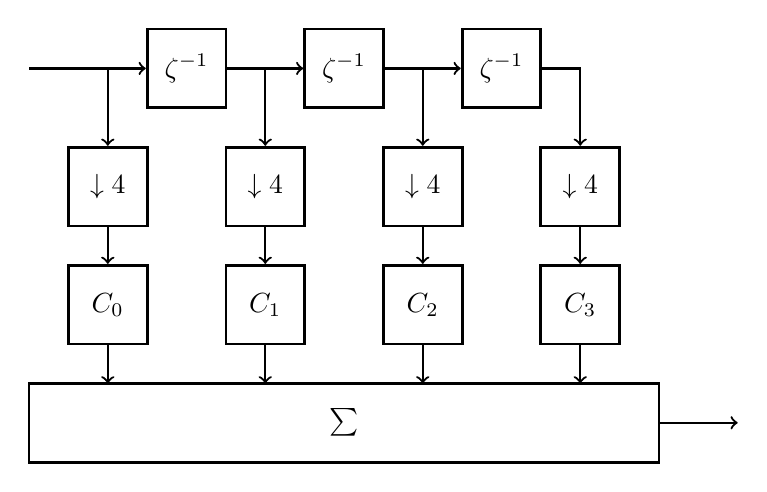
\begin{tikzpicture}
[	
	sq/.style={rectangle,draw,line width=1,minimum height=1cm,minimum width=1cm}
]

\node[sq] (t1) at (1,0) {$\zeta^{-1}$};
\node[sq] (t2) at (3,0) {$\zeta^{-1}$};
\node[sq] (t3) at (5,0) {$\zeta^{-1}$};

\node[sq] (d1) at (0,-1.5) {$\downarrow 4$};
\node[sq] (d2) at (2,-1.5) {$\downarrow 4$};
\node[sq] (d3) at (4,-1.5) {$\downarrow 4$};
\node[sq] (d4) at (6,-1.5) {$\downarrow 4$};

\node[sq] (c1) at (0,-3) {$C_0$};
\node[sq] (c2) at (2,-3) {$C_1$};
\node[sq] (c3) at (4,-3) {$C_2$};
\node[sq] (c4) at (6,-3) {$C_3$};

\node[rectangle,draw,line width=1,minimum height=1cm, minimum width=8cm] (sum) at (3,-4.5) {$\sum$};


\draw[thick,->]	(-1,0)	-- 	(t1);
\draw[thick,->]	(t1)		-- 	(t2);
\draw[thick,->]	(t2) 		-- 	(t3);

\draw[thick,->] (-1,0)	-|	(d1);
\draw[thick,->] (t1)		-|	(d2);
\draw[thick,->] (t2)		-|	(d3);
\draw[thick,->] (t3)		-|	(d4);

\draw[thick,->]	(d1)		-- 	(c1);
\draw[thick,->]	(d2)		-- 	(c2);
\draw[thick,->]	(d3)		-- 	(c3);
\draw[thick,->]	(d4)		-- 	(c4);

\draw[thick,->] (c1) 		-- 	(0,-4);
\draw[thick,->] (c2) 		-- 	(2,-4);
\draw[thick,->] (c3) 		-- 	(4,-4);
\draw[thick,->] (c4) 		-- 	(6,-4);

\draw[thick,->] (sum) -- (8,-4.5);

\end{tikzpicture}